\chapter{Sprint 6 - Summary}
Sprint 6 has mostly been used for documentation refinement and preparation for the second presentation. One week of sprint 6 was also dedicated to exam practice, all exams were finished April 6th and work proceeded on April 7th, giving only 2 workdays and a weekend for further technical work.  \\

When testing the variable pitch quadcopter, one of the servos was fried. The servos movement was also considered to be too twitchy for precise pitch control. New high quality servos were ordered from Elefun, with no-load speed of 0,04 s/60 degrees (8,4V), in comparison to the current with no-load speed of 0,07 s/60 degrees (6V) and poor build quality. \\
 
For the quadcopter, a radio controller was implemented (Fig. \ref{fig:radio}) and flight testing with radio control will start at the beginning of sprint 7. In parallel the autonomous control system is being developed for integration with Qualisys. 

\begin{figure}[H]
    \centering
         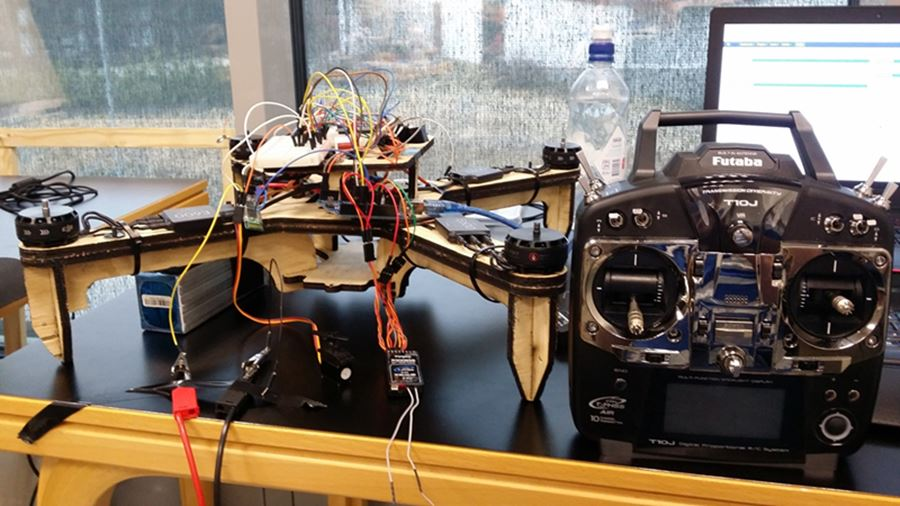
\includegraphics[width = 1\textwidth]{VAPIQ-PICTURES/radiocontroller}
      \caption{Radio Controller with the Plywood Quadcopter}
    \label{fig:radio}
\end{figure} 



\clearpage

\section{Completion and Scope Change}

In sprint 6, 88\% of tasks were completed and no changes in scope.


\begin{figure}[H]
    \centering
         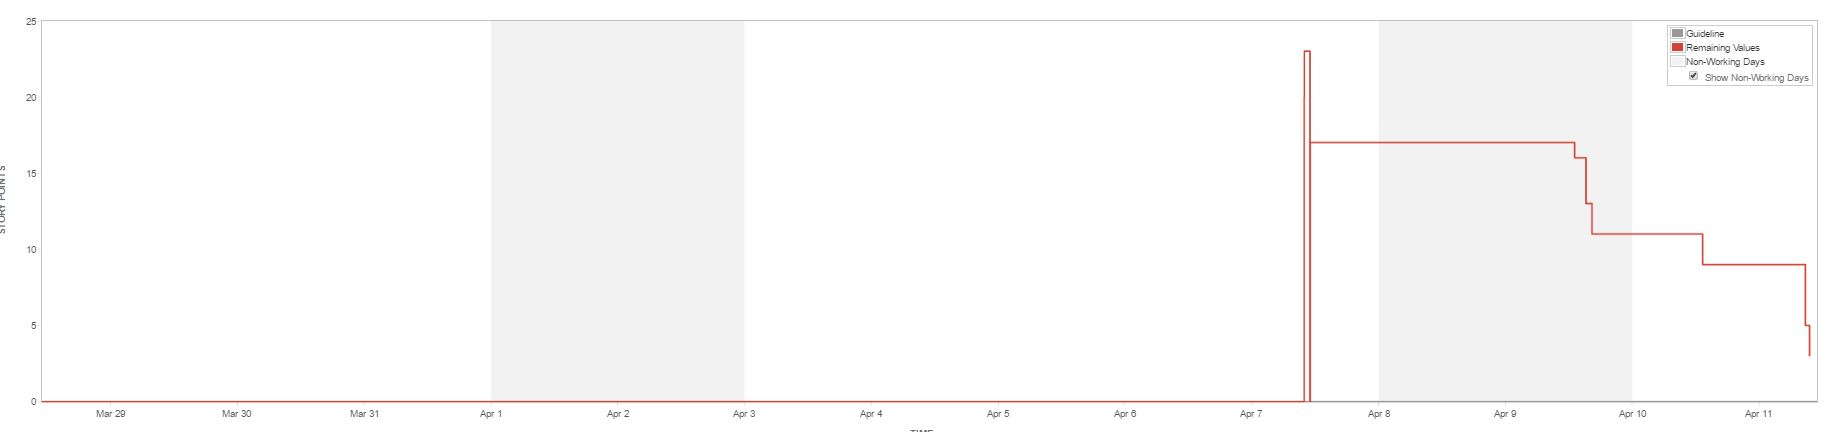
\includegraphics[width = 1\textwidth]{VAPIQ-PICTURES/BDSprint6}
      \caption{Burndown Chart,Sprint 6}
    \label{fig:bd6}
\end{figure} 

\textbf{Project plan status, Sprint 6:}
\begin{itemize}
        \item Exam In Other Subjects \textbf{Done}
        \item Plan Research Strategy and Methodology \textbf{In progress}
        \item Electrical Construction VPQ \textbf{Done}
        \item Control System, \textbf{Done}
        \item Basic Flight Controller, VPQ, \textbf{Done}
    \end{itemize}


%\subsection{Results and Conclusions}

%New servos has been acquired and the variable pitch quadcopter has been fully assembled with the new servos.

%This sprint has been the shortest sprint yet, and there was little time left for further technical work. Some time was used in this sprint to properly plan for the upcoming sprint 7.

%skriv mer-------------------------------------------------------
		




\begin{comment}
Ting å få med: 

Presentation 2 
Exam
Sprint planning for Sprint 7
Radio Controller 
New Servos from Elefun ordered
Variable Pitch Quadcopter assembled and soldered 

Assembly VPQ
Code progress VPQ
Flight test

						
\end{comment}